\documentclass{beamer}
\usepackage[spanish]{babel}
\usepackage{graphicx}
\usepackage{tema-computadora}

% ruta donde estan las imagenes, relativa a este archivo (diapos/diapos.tex)
% asi en \includegraphics no hay que escribir "../imagenes/" cada vez
\graphicspath{{../imagenes/}}

\title{Popusintesíntesis}
\subtitle{Presentación candidatura de doctorado}
\author{Aarón Montoya Moraga}
\institute{Universidad de Santiago de Chile \\ Instituto de Estudios Avanzados}
\date{\today}

\begin{document}

\frame{\titlepage}

\begin{frame}{Índice}
  \tableofcontents
\end{frame}

\section{Introducción}

\begin{frame}{Introducción}
  Placeholder.
\end{frame}

\section{Metodología}

\begin{frame}{Metodología}
  Placeholder.
\end{frame}

\section{Prototipos}

\begin{frame}{Módulo Relo}
  \centering
  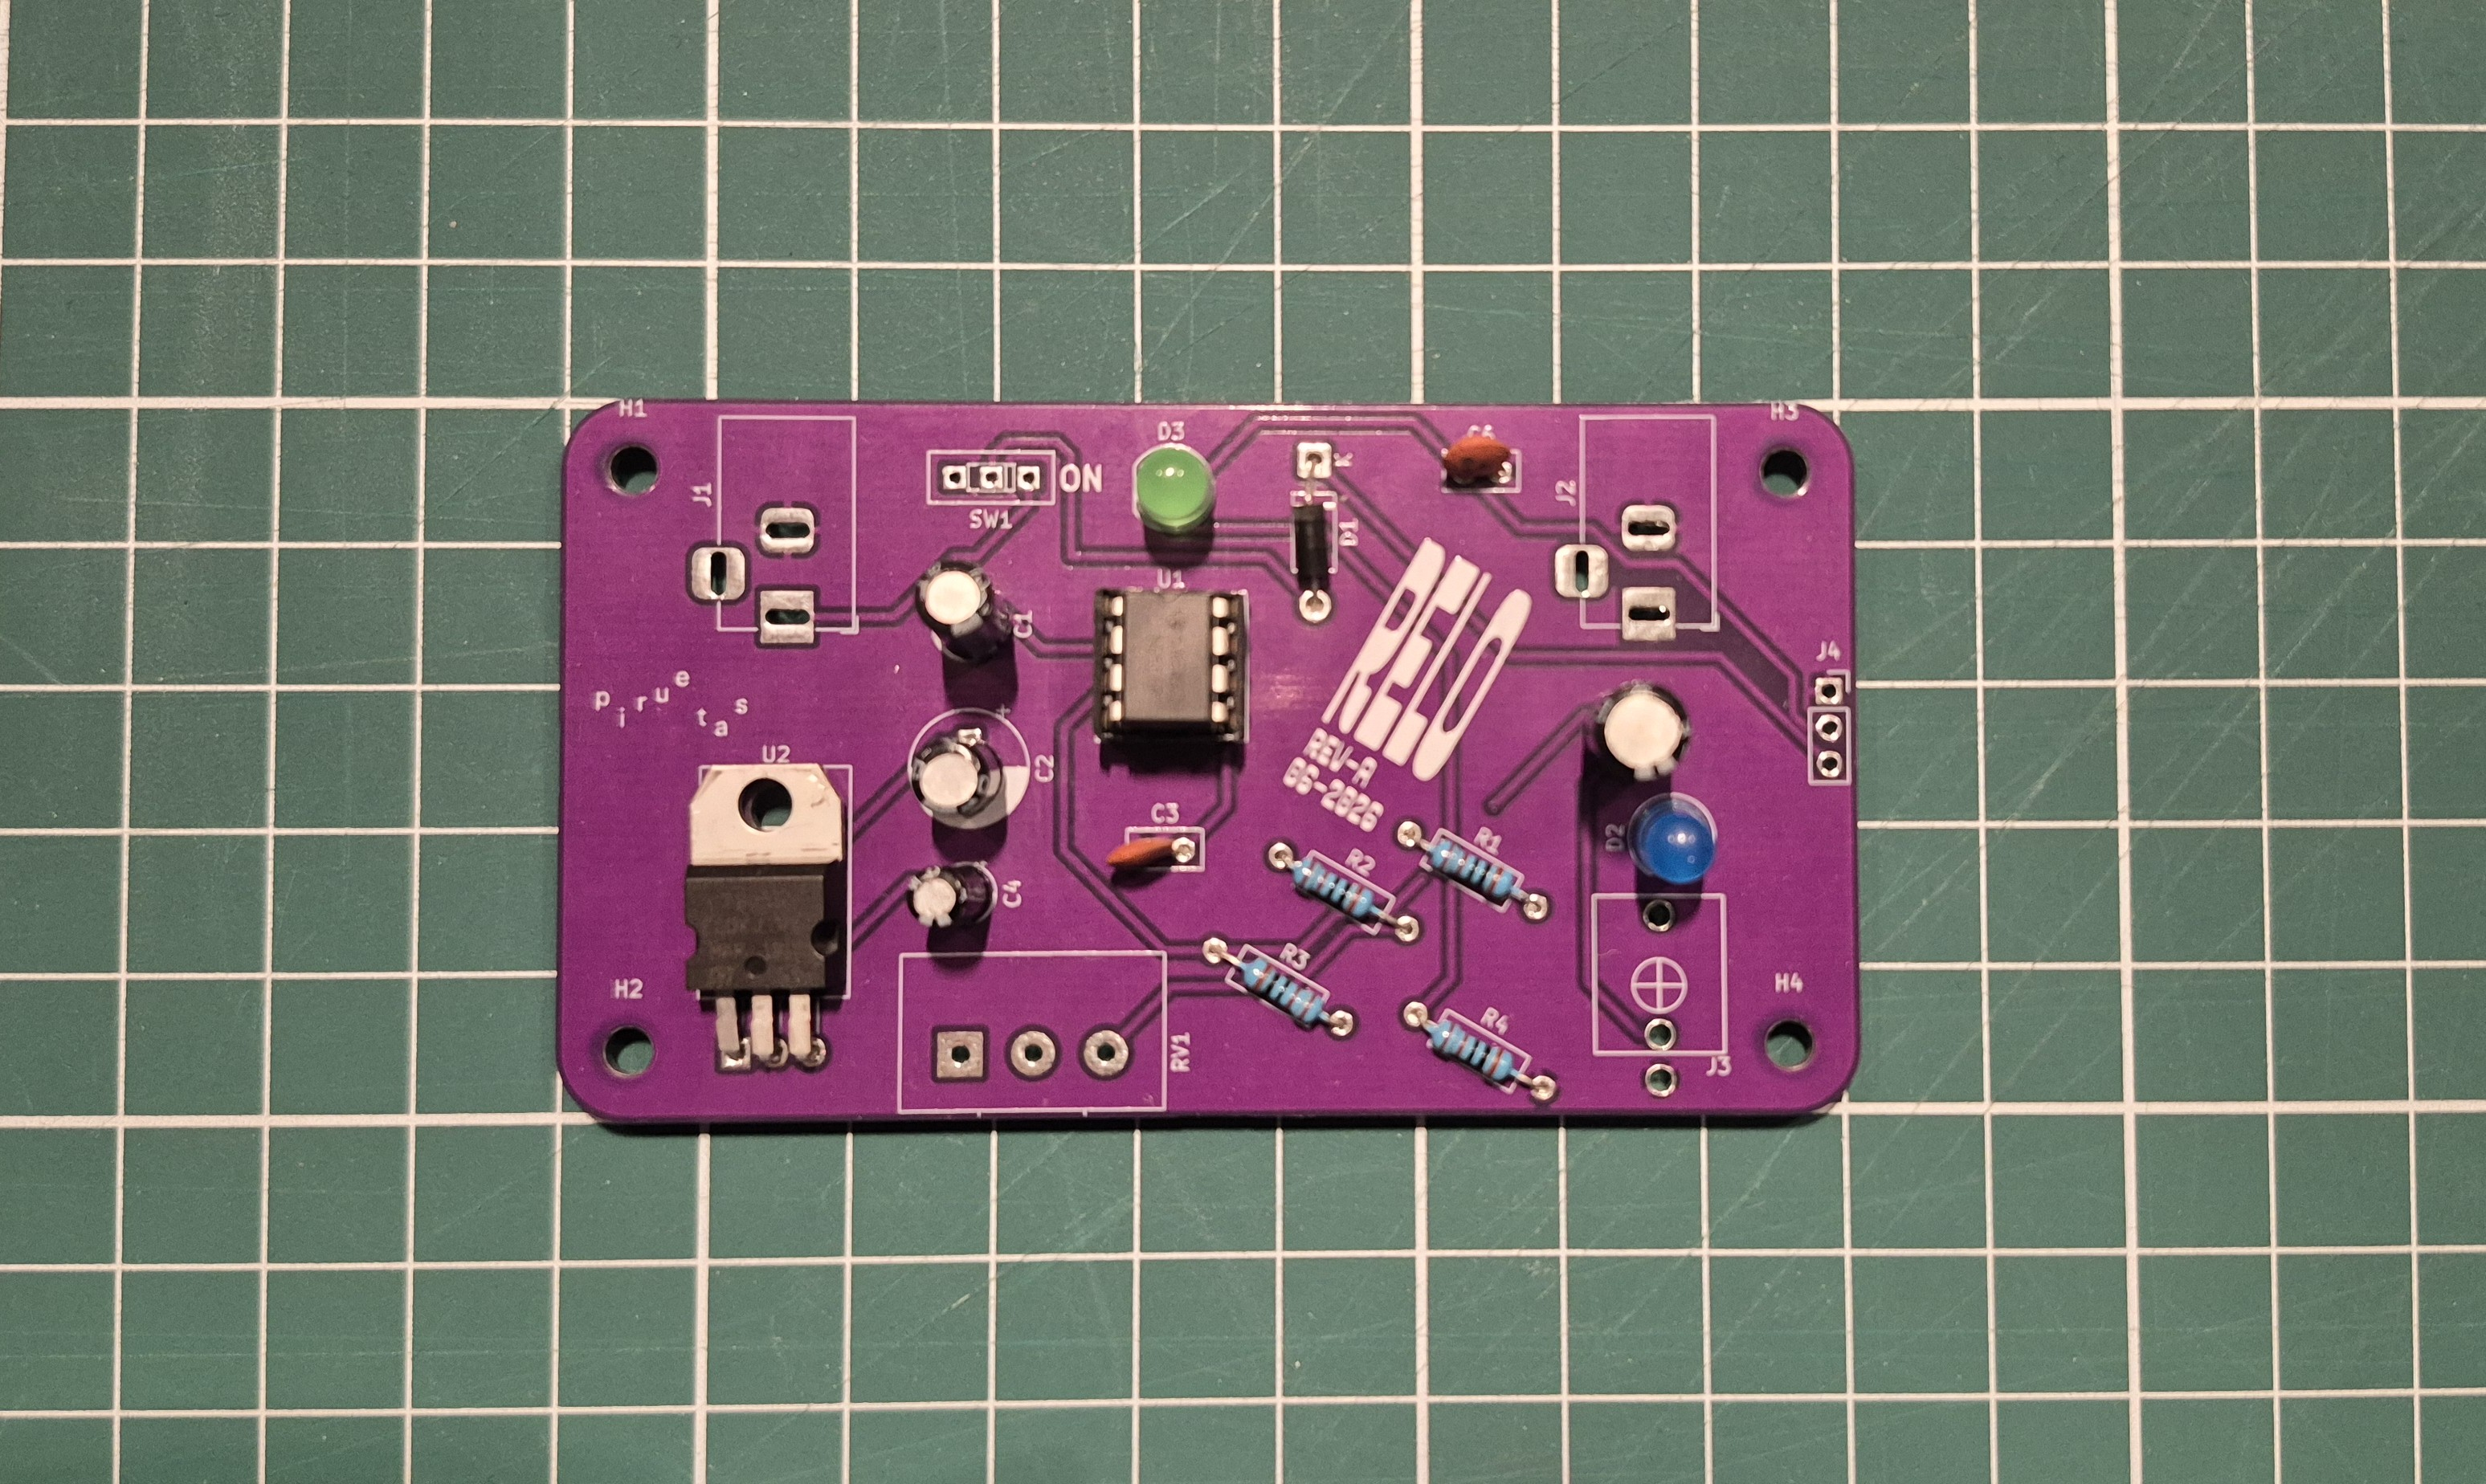
\includegraphics[width=0.6\textwidth]{relo-v0.jpg}

  Placa soldada del módulo Relo.
\end{frame}

\begin{frame}{Módulo Parla}
  \begin{columns}
    \column{0.5\textwidth}
      \centering
      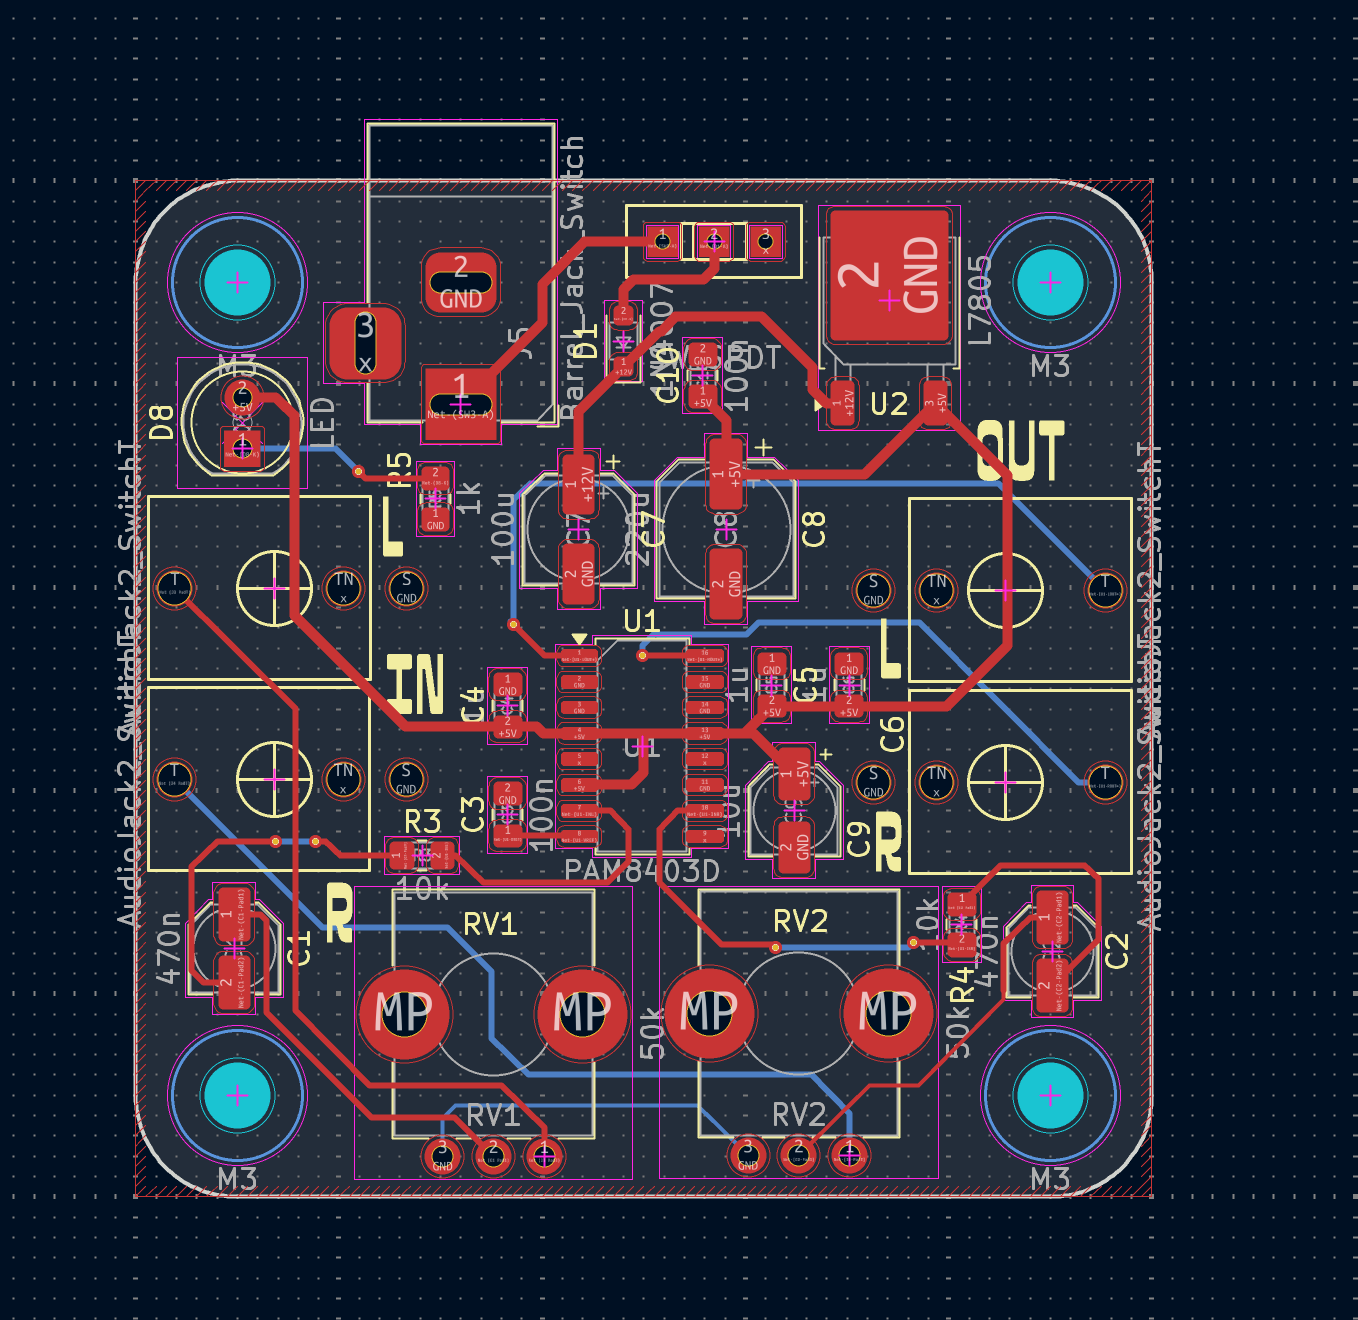
\includegraphics[width=\linewidth]{parla-v0-rev-b-pcb.png}

      Placa diseñada
    \column{0.5\textwidth}
      \centering
      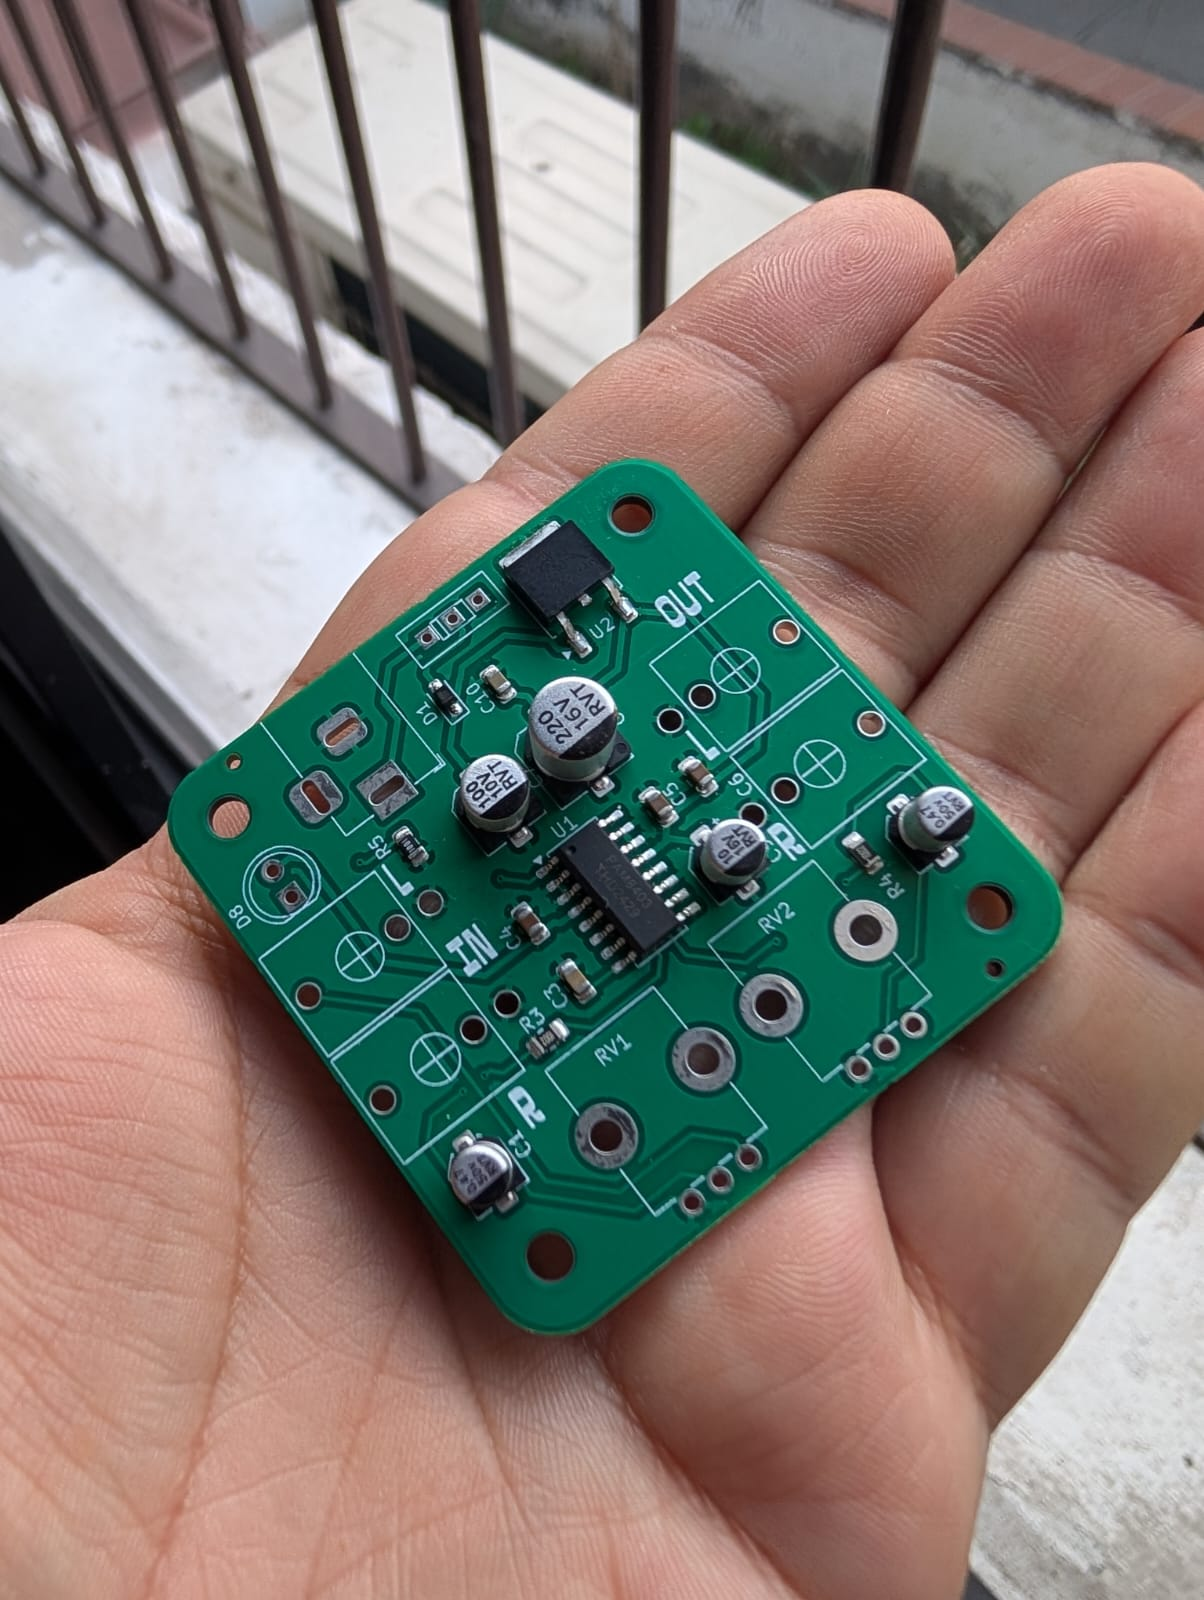
\includegraphics[width=\linewidth]{parla-v0-rev-b.jpg}

      Placa construida
  \end{columns}
\end{frame}

\begin{frame}{Módulo Parla: esquemático}
  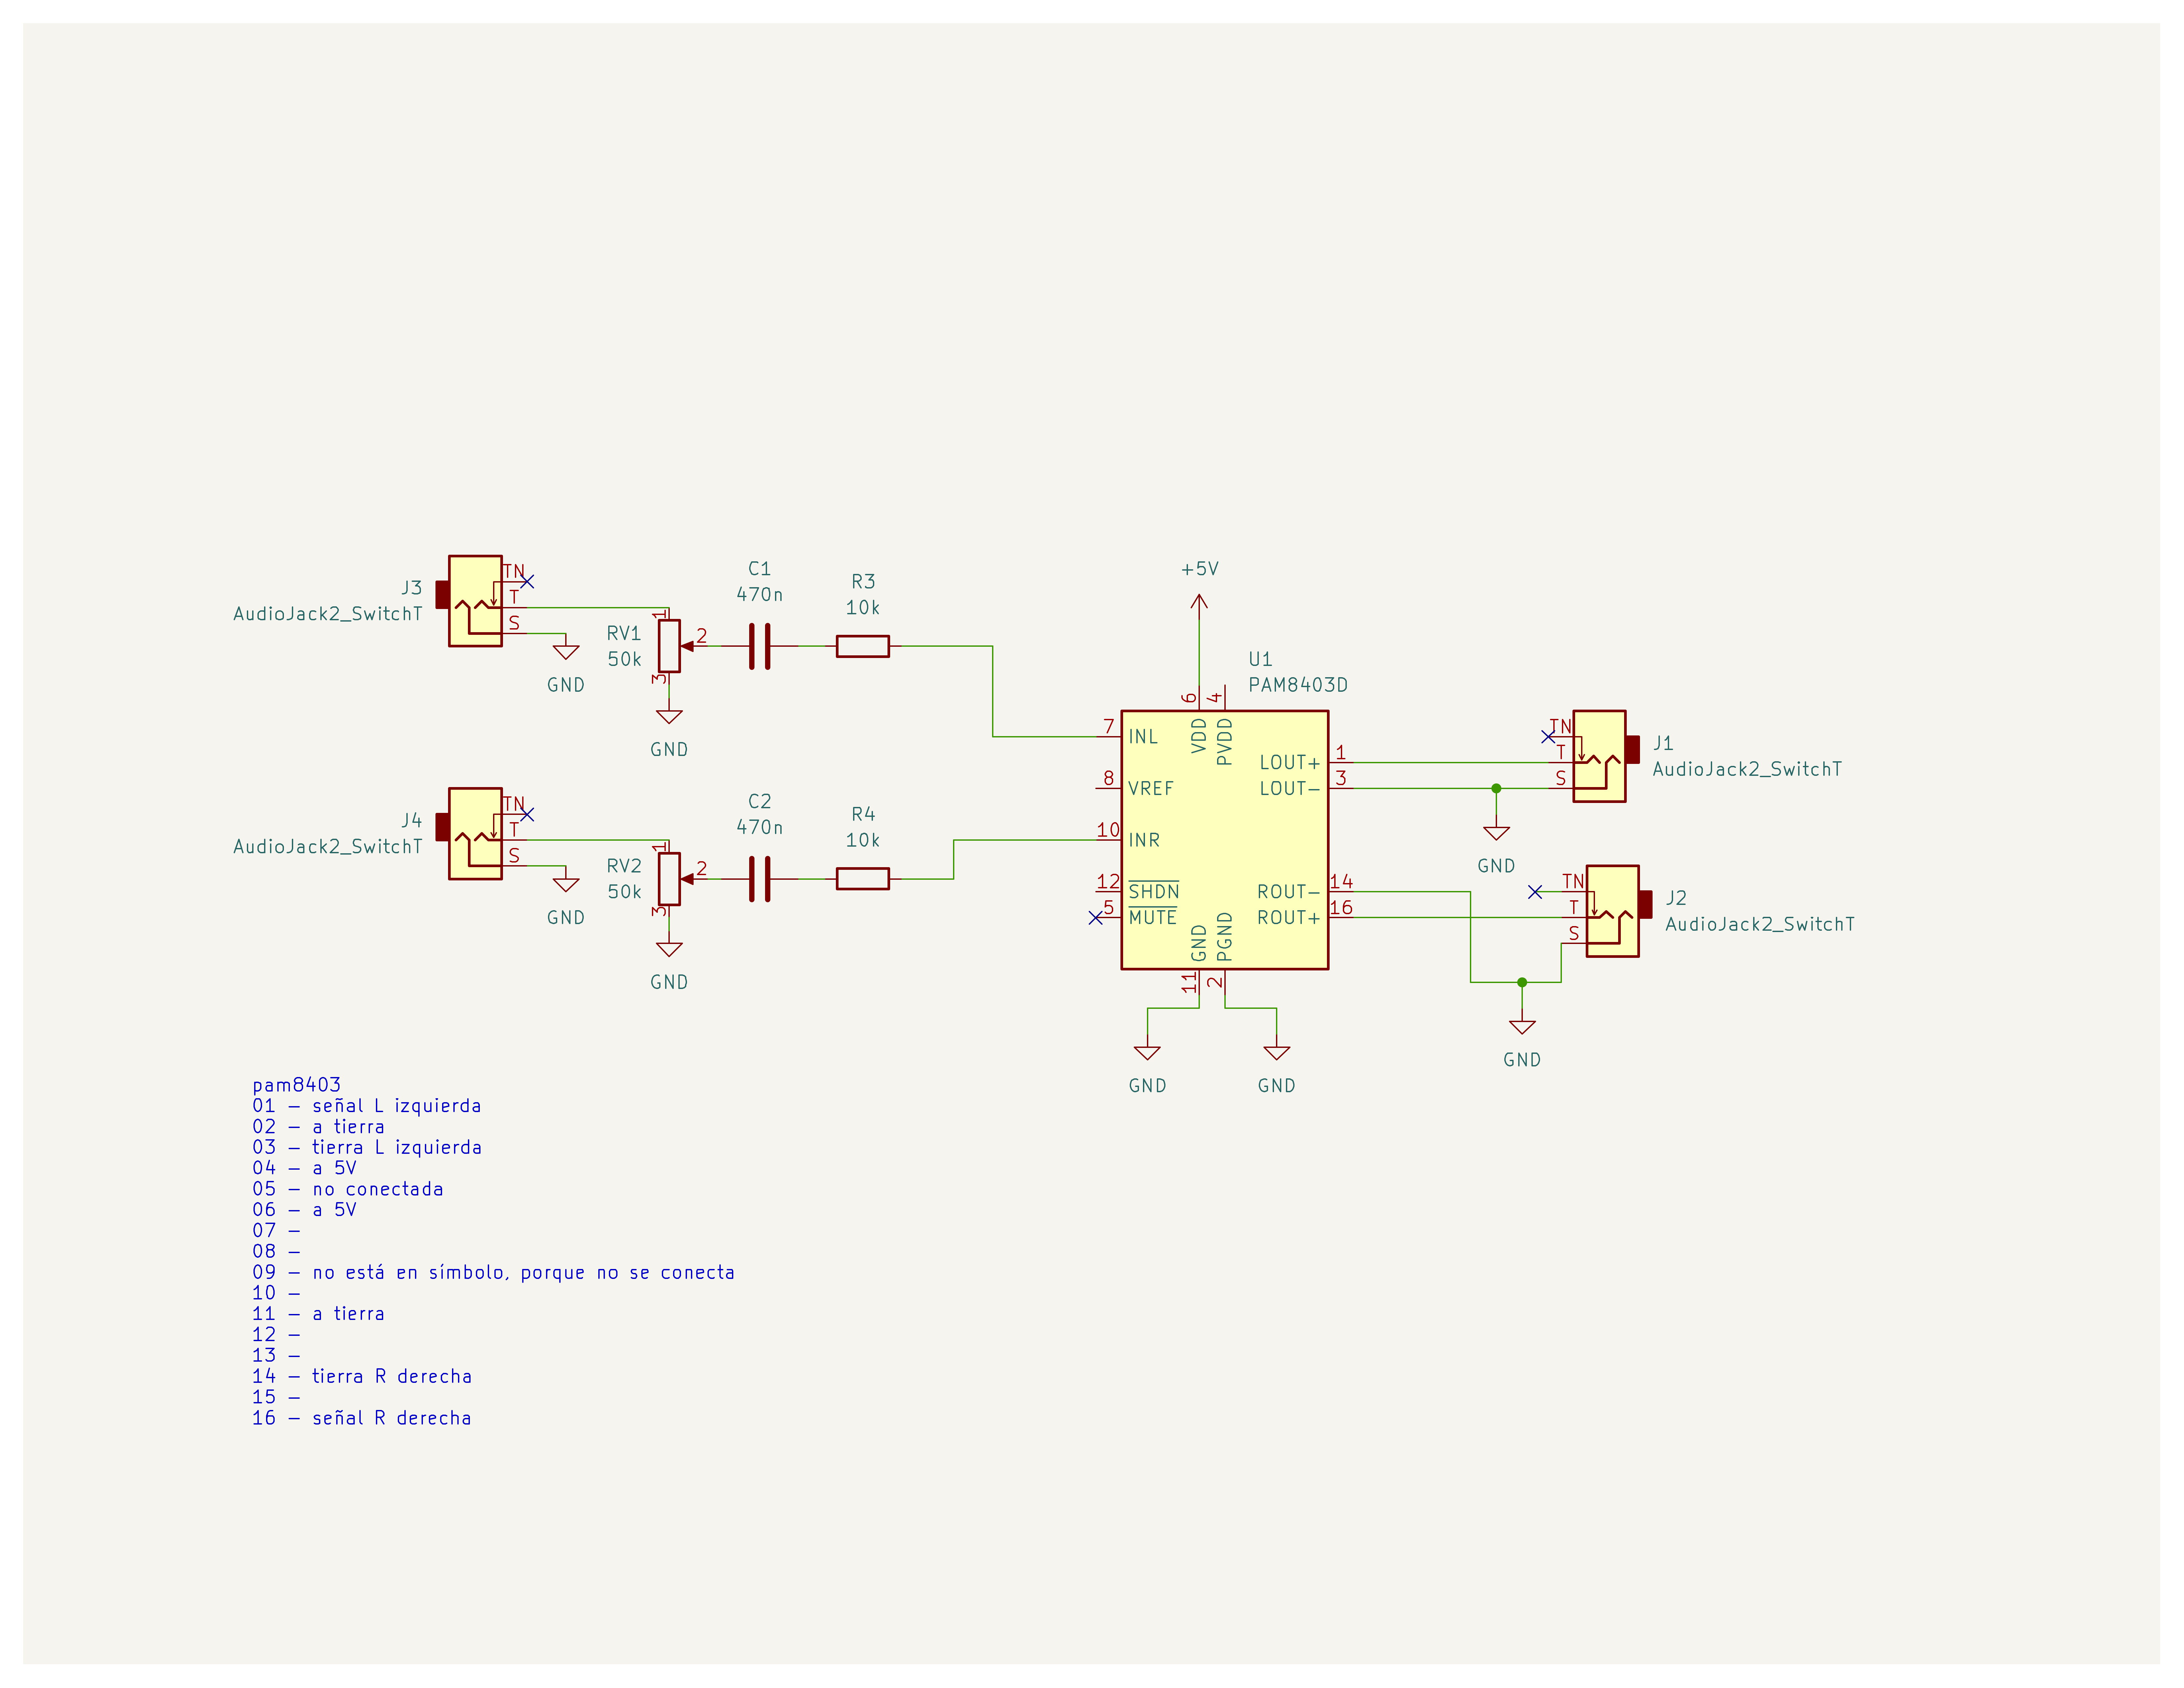
\includegraphics[width=0.5\textwidth]{parla-v0-rev-b-sch.png}
  \hfill
  \begin{minipage}{0.45\textwidth}
    \begin{itemize}
      \item Primera iteración (enero 2026): mono, chip LM386.
      \item Segunda iteración (junio 2026): estéreo, chip PAM8403D.
    \end{itemize}
  \end{minipage}
\end{frame}

\section{Resultados esperados}

\begin{frame}{Resultados esperados}
  Placeholder.
\end{frame}

\end{document}
